
\subsection{Components}

In this subsection, we numerically benchmark the spacetime cost of LOBE constructions for three different sets of operators.
We compare the cost of the constructions with the two methods outlined above which require expanding the ladder operators in the Pauli basis.

\begin{figure*}
    \centering
    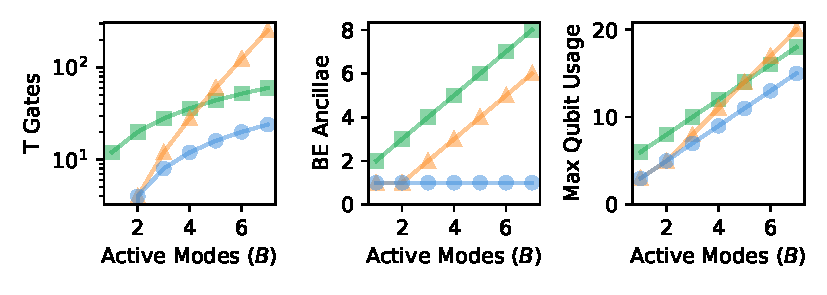
\includegraphics[width=12cm]{figures/fermionic-hc-comparison.pdf}
    \caption{
        \textbf{Spacetime Cost to Block-Encode $O = b_0 b_1 \hdots b_{B-1} + h.c.$}
        The number of T gates (left), block-encoding ancillae (middle), and maximum number of qubits used (right) are shown as a function of the number of active modes ($B$).
        Results for ``Pauli Expansion'' are shown as the orange triangles, results for ``Piecewise Pauli'' are shown as the green squares, and results for LOBE are shown as the blue circles.
        For this operator, all block-encodings use zero non-Clifford rotations.
        Both ``Pauli Expansion'' and LOBE have optimal rescaling factors ($\lambda = 1$) while ``Piecewise Pauli'' has a rescaling factor of $\lambda = 2$.
    }
    \label{fig:fermionic-hc-comparison}
\end{figure*}

The first set of operators we examine are described by a product of fermionic annihilation operators acting on different modes plus its hermitian conjugate: $b_0 b_1 \hdots b_{B-1} + h.c.$.
The numerical spacetime costs of the three block-encoding methods for these operators are shown as a function of the number of active modes ($B$) in Figure \ref{fig:fermionic-hc-comparison}.
Notably, the spacetime costs for LOBE and ``Pauli Expansion'' are identical for $B = 1$ and $B = 2$.
However, the number of required T gates scales exponentially with $B$ for ``Pauli Expansion'', yet scales linearly for LOBE.
Additionally, the LOBE constructions only require a single block-encoding ancilla, independent of $B$,while both Pauli-based methods require a number of block-encoding ancillae that scale linearly with $B$.

\begin{figure*}
    \centering
    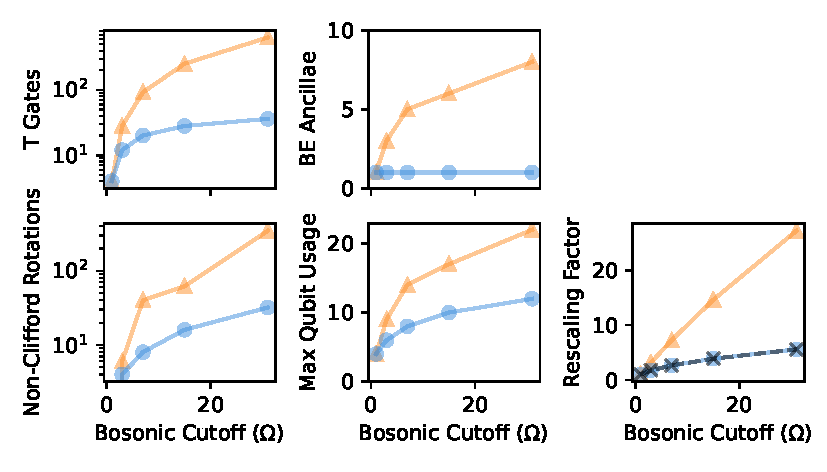
\includegraphics[width=14cm]{figures/bosonic-comparison.pdf}
    \caption{
        \textbf{Spacetime Cost to Block-Encode Bosonic Annihilation Operator}
        The number of T gates (upper-left), number of non-Clifford rotations (lower-left), block-encoding ancillae (upper-middle), maximum number of qubits used (lower-middle), and rescaling factor (lower-right) are shown as a function of the bosonic occupation cutoff ($\Omega$).
        Results for the Pauli (LCU) method are shown as the orange triangles and results for LOBE are shown as the blue circles.
        The optimal rescaling factor, which is given by the L2 norm of the matrix representing the bosonic annihilation operator with fixed $\Omega$, is shown as the dashed black crosses. 
    }
    \label{fig:bosonic-comparison}
\end{figure*}

The second set of block-encodings we consider is those that encode a single bosonic annihilation operator ($a$) with an increasing bosonic occupation cutoff ($\Omega$).
Since there is only a single operator, both Pauli methods result in the same construction therefore we refer to these constructions by ``Pauli (LCU)''.
The numerical spacetime costs and rescaling factors of the Pauli (LCU) and LOBE block-encodings are shown in Figure \ref{fig:bosonic-comparison}.
The LOBE constructions result in block-encodings with fewer required resources for all metrics as compared to the Pauli (LCU) method.
Notably, the number of required T gates scales logarithmically with $\Omega$ for LOBE, yet scales roughly linearly for the Pauli (LCU) method.
Additionally, the number of block-encoding ancillae is constant ($1$) regardless of $\Omega$ for LOBE, yet scales logarithmically for the Pauli (LCU) method.
Lastly, the LOBE construction results in a rescaling factor that matches the operator norm (optimal), while the Pauli (LCU) construction results in a larger rescaling factor.

\begin{figure*}
    \centering
    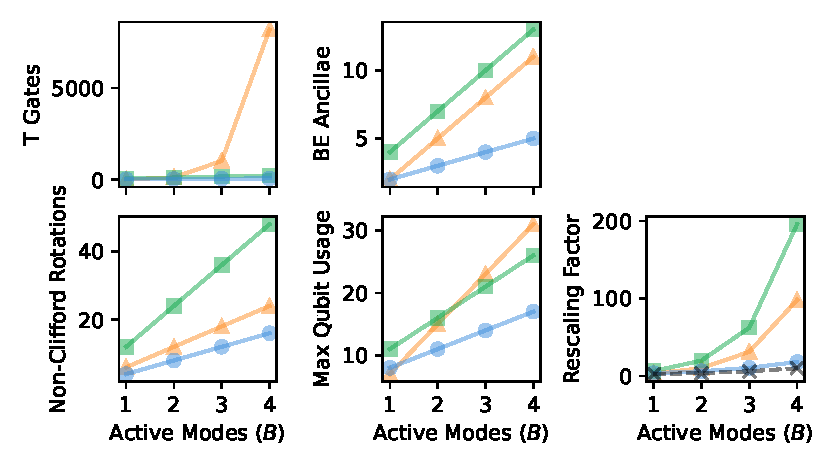
\includegraphics[width=14cm]{figures/bosonic-hc-comparison.pdf}
    \caption{
        \textbf{Spacetime Cost to Block-Encode $O = a_0 a_1 \hdots a_{B-1} + h.c.$}
        The number of T gates (upper-left), number of non-Clifford rotations (lower-left), block-encoding ancillae (upper-middle), maximum number of qubits used (lower-middle), and rescaling factor (lower-right) are shown as a function of the number of active modes ($B$).
        The bosonic cutoff is fixed to $\Omega = 3$ for all data points.
        Results for ``Pauli Expansion'' are shown as the orange triangles, results for ``Piecewise Pauli'' are shown as the green squares, and results for LOBE are shown as the blue circles.
        The optimal rescaling factor, which is given by the L2 norm of the matrix representing the operator with $\Omega = 3$, is shown as the dashed black crosses.
    }
    \label{fig:bosonic-hc-comparison}
\end{figure*}

The third set of operators we analyze are given as a linear combination of a product of bosonic annihilation operators acting on different modes plus its hermitian conjugate: $a_0 a_1 \hdots a_{B-1} + h.c.$.
The numerical spacetime costs of the various block-encoding constructions for these operators with $\Omega = 3$ are shown in Figure \ref{fig:bosonic-hc-comparison}.
Notably, the overall time-complexity scales linearly with $B$ for the LOBE and ``Piecewise Pauli'' constructions, while it scales exponentially for ``Pauli Expansion''.
For the space complexity metrics, all methods scale linearly with $B$, yet the LOBE constructions have both the smallest prefactor and numerical values.
Finally, the LOBE construction results in the lowest rescaling factor of all constructions.

In certain cases - such as when the number of active modes is small or the bosonic occupation cutoff is low - the ``Pauli Expansion'' construction can lead to lowest spacetime costs.
However, when the number of active modes is large or the bosonic occupation cutoff is high, the LOBE constructions lead to the lowest spacetime costs.
For all components analyzed here, the ``Piecewise Pauli'' constructions have similar asymptotic scalings compared to LOBE, but result in larger numerical spacetime costs.
For this reason, the ``Piecewise Pauli'' construction will be omitted when benchmarking full systems.
